\chapter{Эксперимент PHENIX} \label{chapt2}

\section{Коллайдер релятивистских тяжелых ионов (RHIC)} \label{sect2_RHIC}
Релятивистский коллайдер тяжелых ионов RHIC (англ. The Relativistic Heavy Ion Collider) \cite{RHIC}, расположенный в Брукхейвенской национальной лаборатории, штат Нью-Йорк, является первым и одним из двух действующих коллайдеров тяжелых ионов и единственным из когда-либо построенных спин-поляризованных протонных коллайдеров. 
Коллайдер RHIC предназначен для столкновения ионов, движущихся с релятивистскими скоростями, и изучения кварк-глюонной плазмы --  первичной формы материи, которая существовала во вселенной в первые доли секунды после Большого взрыва. При столкновении спин-поляризованных протонов исследуется спиновая структура протона.
В настоящее время RHIC является вторым по значению достигаемой энергии в системе центра масс (\sqsn = 200 ГэВ) коллайдером тяжелых ионов в мире после Большого адронного коллайдера (LHC) (\sqsn = 6,5 ТэВ).

\begin{figure}[ht] 
	\centerfloat
	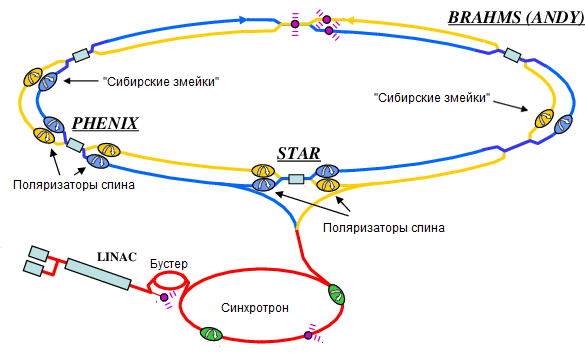
\includegraphics [width = 1\linewidth] {PHENIX/RHIC.png}
	\caption{Схема ускорительного комплекса коллайдера RHIC} 
	\label{img:RHIC}  
\end{figure}

Ускорительный комплекс коллайдера RHIC состоит из: источника ионов, линейного ускорителя (LINAС), ускоряющего синхротрона (бустера), синхротрона и двух колец коллайдера RHIС.

%/* PHENIX-diss*/

Схема установки RHIC показана на Рисунке \ref{img:RHIC}. Пучки сталкивающихся ионов предварительно ускоряются с помощью ускорителя Ван де Граафа до энергии 1 МэВ/нуклон, а затем синхротроном-бустером до энергии 192 МэВ/нуклон, после чего инжектируются в кольцо синхротрона с переменным градиентом (AGS). Далее пучки сталкивающихся ионов, ускоренные AGS до 10,8 ГэВ, инжектируются в основное колбцо коллайдера RHIC. Инжектированные пучки сталкивающихся ионов ускоряются до 100 ГэВ/нуклон в кольце RHIC и сталкиваются в в одной из шести точек взаимодействия пучков.

На коллайдере RHIC располагаются 4 эксперимента: PHENIX, STAR, PHOBOS и BRAMS. В настоящее время все эксперименты, кроме эксперимента STAR, закончили свою работу. Детектор PHENIX завершил набор новых данных в 2017 г, однако обработка уже полученных данных ведется по сей день. В данной работе использованы данные, полученные в эксперименте PHENIX в 2012, 2014 и в 2016 гг.



\section{Эксперимент PHENIX}

PHENIX (Pioneering High Energy Nuclear Interaction eXperiment) \cite{PHENIXoverview, PHENIXoverview2} является экспериментом по исследованию столкновений тяжелых ионов и протонов высоких энергий. Основная задача эксперимента PHENIX состоит в изучении кварк-глюонной плазмы, образующейся в столкновениях тяжелых релятивистских ионов. 

\begin{figure}[ht] 
	\centerfloat
	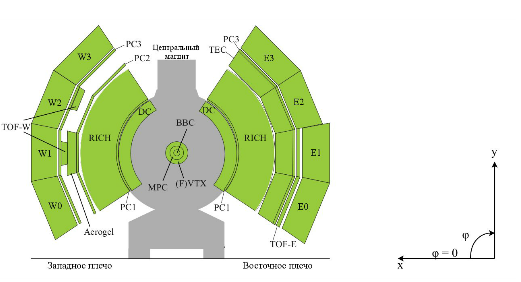
\includegraphics [scale = 0.9] {PHENIX/PHENIX_EXP.png}
	\caption{Схема эксперимента PHENIX} 
	\label{img:PHENIX_EXP}
\end{figure}
\begin{figure}[ht] 
	\centerfloat
	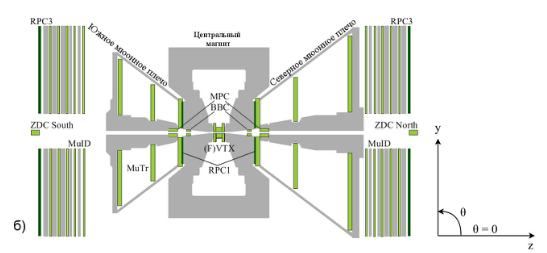
\includegraphics [scale = 0.9] {PHENIX/PHENIX_EXP2.png}
	\caption{Схема эксперимента PHENIX} 
	\label{img:PHENIX_EXP2}
\end{figure}


Эксперимент PHENIX состоит из 12 детекторных систем, которые сгруппированы в четыре основных блока, называемых плечами. Схематическое изображение эксперимента PHENIX представлено на Рисунке \ref{img:PHENIX_EXP}. Центральные плечи – восточное и западное – предназначены для регистрации лептонов, фотонов и заряженных адронов. Три стальных магнита (центральный и два мюонных) создают магнитные поля удерживающие заряженные частицы внутри кольца ускорителя.
Детекторы, использованные в данной работе описаны ниже.

\subsection{Дрейфовые камеры}
Дрейфовые камеры (ДК) являются проволочными газонаполненными ионизационными детекторами, предназначенными для измерения поперечного импульса и траектории заряженных частиц в плоскости полярного угла $\varphi$. 
ДК расположены зеркально в западном и восточном плече на расстоянии 200 см от центра столкновения.

ДК имеет многопроволочную структуру (12800 считывающих проволочек) и состоит из модулей (Рисунок \ref{img:PHENIX_DC}).
Модуль ДК представляет собой титановый каркас с двумя майларовыми окнами, заполненный проволками шести типов: X1, U1, V1, X2, U2, V2. Проволоки различных типов объединены в проволочные плоскости X, U и V соответственно. 
Проволочная плоскость X является анодной и содержит 12 проволок расположенных вдоль оси $z$. Плоскость X служит для измерения азимутального угла трека частиц $\varphi$, а также угла $\alpha$ между радиус-ветором  и касательной к треку частицы в точке, равной эталонному радиусу ДК $r_{DC} = 220$ см. (Рисунок \ref{img:PHENIX_DCtracks} а))
За плоскостью проволок X следуют два набора проволочных плоскостей  U и V, расположенных под небольшим углом относительно оси $z$, предназначенных для определения координаты частицы в плоскости $z -- r$ вдоль оси $z$ -- $zed$ (Рисунок \ref{img:PHENIX_DCtracks} б)). 
\begin{figure}[ht] 
	\centerfloat
	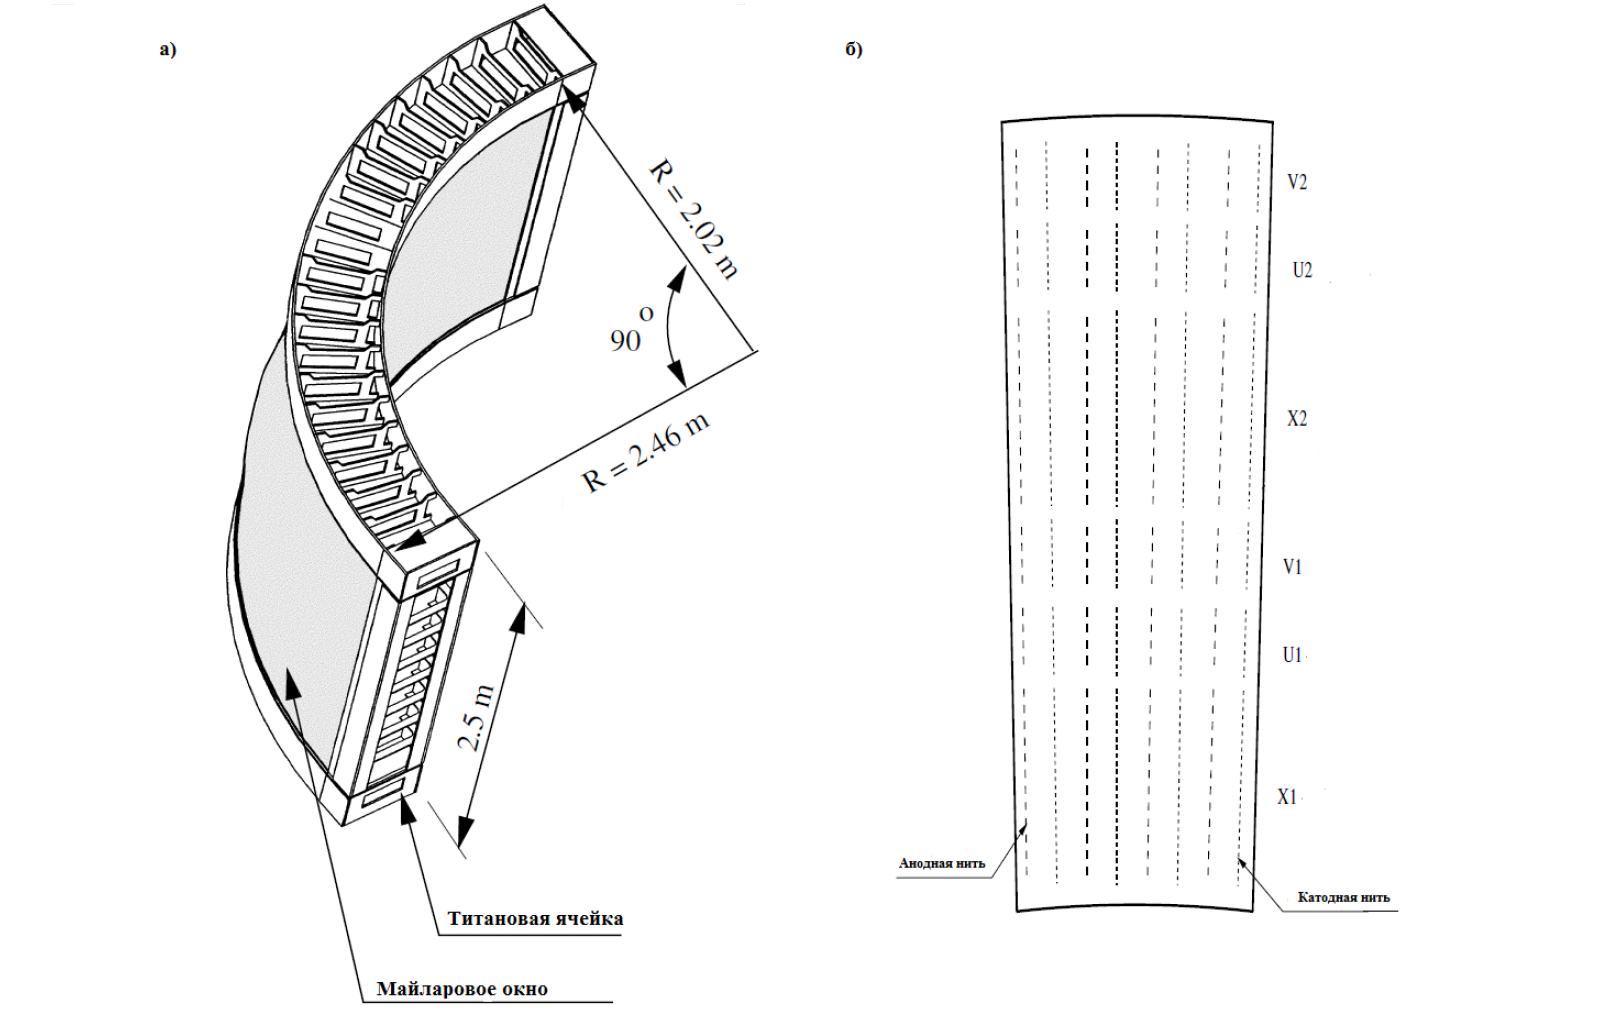
\includegraphics [scale = 0.4] {PHENIX/DC.png}
	\caption{Схема модуля дрейфовой камеры} 
	\label{img:PHENIX_DC}
\end{figure}

\begin{figure}[ht] 
	\centerfloat
	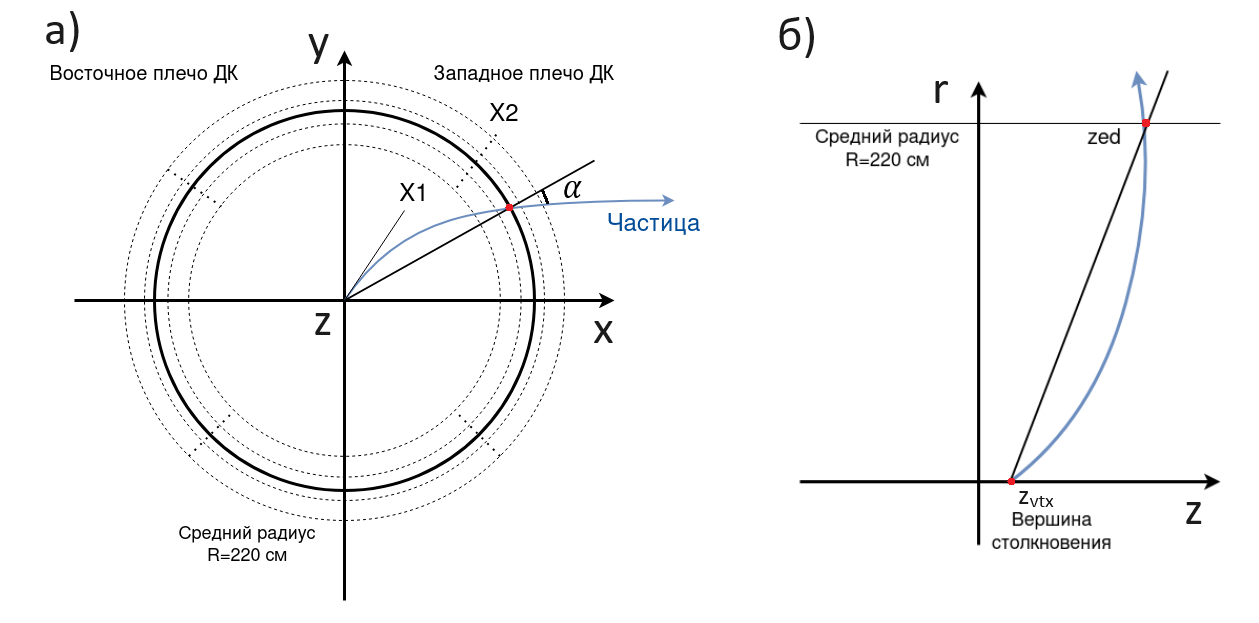
\includegraphics [width=0.9\linewidth]{PHENIX/DC_tracks.png}
	\caption{Схема модуля дрейфовой камеры} 
	\label{img:PHENIX_DCtracks}
\end{figure}

Степень точности определения треков частиц характеризуется битом качества отслеживания $Q_{track}$. Наилучшие степени точности восстановления трека соответствуют величинам $Q_{track}$ равным 63, 31 и 51.
 
\begin{comment}
\textcolor{red}{
Из-за несовершенства геометрии центральной трековой системы и ее ка­либровок один и тот же трек заряженной частицы может быть восстановлен дважды. В этом случае оба трека будут иметь близкие значения координаты $z$ и азимутального угла $\varphi$. Для исключения подобных пар треков из анализа
используются критерии отбора, приведенные в Таблице 6.
$zed$ – координата по оси $z$, при которой трек имеет радиус-вектор $r_{track} = r_{DC}$.
}
\end{comment}

\subsection{Падовые камеры}
Падовые камеры (ПК) представляют собой многопроволочные пропорциональные камеры, которые образуют три отдельных слоя центральной трекинговой системы PHENIX. 
На Рисунке \ref{img:PHENIX_PC} показано расположение ПК в центральных плечах эксперимента PHENIX. Первый слой падовых камер (ПК1) расположен сразу после дрейфовых камер, т.е. на расстоянии 2,49 м от точки взаимодействия, третий слой (ПК3) — на расстоянии 4,98 м от точки взаимодействия. Второй слой (ПК2) расположен на радиальном расстоянии 4,19 м от точки взаимзаимодействия только в западном плече.

Каждая ПК содержит анодную проволочную плоскость внутри газового объема, ограниченного двумя катодными плоскостями, одна из которых сегментирована в массив пикселей. При прохождении ионизирующей частицы через камеру, электроны, образованные в результате ионизации, начинают дрейфовать по направлению к анодным проволокам. В непосредственной близости от анодной нити, где напряженность электрического поля достаточно велика, электрон начинает ионизовывать молекулы газа, образуя лавину. Заряд, индуцированный лавиной на пикселях ПК регистрируется считывающей электроникой. 

Расстояние между анодными проволоками составляет 8,4 мм, площадь ячейки -- 8,4 × 8,4 мм$^2$. Данная геометрия обеспечивает координатное разрешение ±1,7 мм. ПК2 и ПК3 должны иметь разрешение не хуже, чем ПК1. Таким образом, ячейки ПК3 имеют в 4 раза большую площадь, чем ячейки ПК1, поскольку ПК3 находится в два раза дальше от вершины столкновения, чем ПК1.

\begin{figure}[ht] 
	\centerfloat
	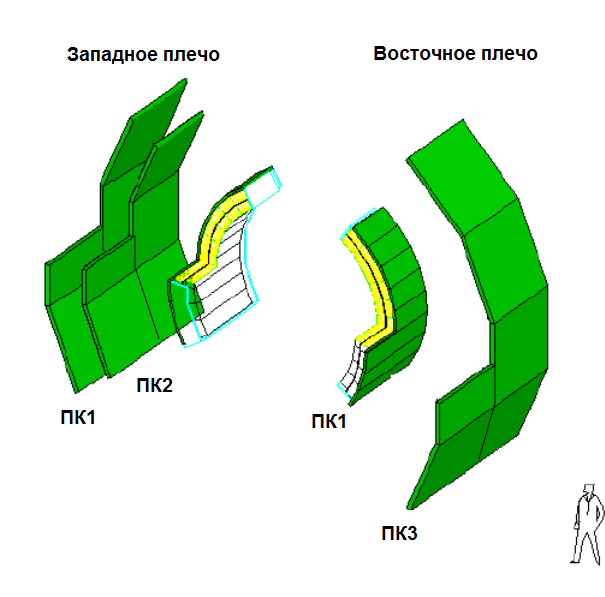
\includegraphics [scale = 0.6] {PHENIX/PC.png}
	\caption{Расположение падовых камер в центральных плечах эксперимента PHENIX.} 
	\label{img:PHENIX_PC}
\end{figure}


\begin{figure}[ht] 
	\centerfloat
	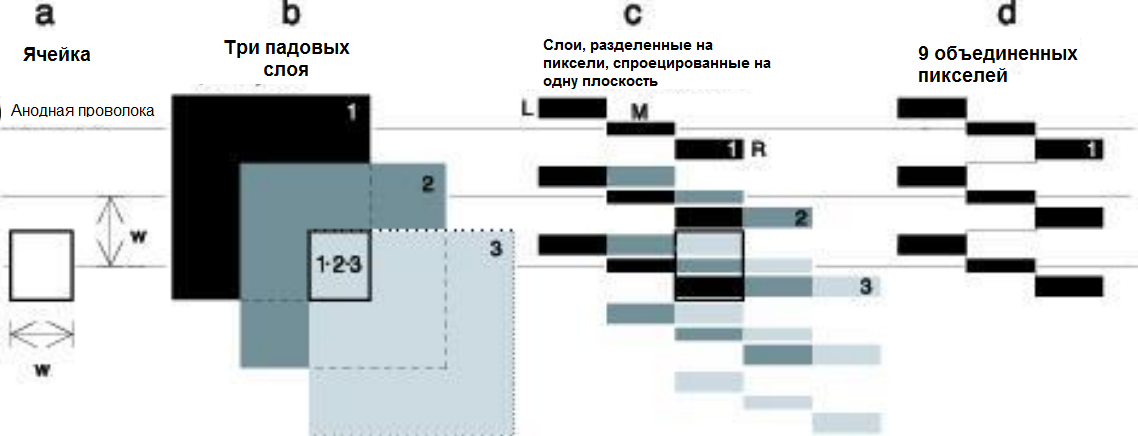
\includegraphics [scale = 0.5] {PHENIX/PC_2.png}
	\caption{Схема ячеек падовых камер} 
	\label{img:PHENIX_PC2}
\end{figure}

На Рисунке \ref{img:PHENIX_PC2} показана схема ПК. ПК состоит из ячеек, каждая из которых содержит три пикселя. Лавина регистрируется только в случае регистрации сигнала в каждом из пикселей ячейки. Каждые девять пикселей, составляющих три ячейки, объединены и подключены к общему каналу считывания таким образом, что три пикселя в ячейке всегда связаны с разными, но соседними каналами. В таком случае каждая ячейка определяется своей уникальной тройкой каналов. Данная структура падовых камер позволяет уменьшить количество каналов считывания в девять раз по сравнению со схемой считывания каждого пикселя и в три раза по сравнению с схемой считывания каждой ячейки. 

\subsection{Времяпролетная камера}
Времяпролетная камера (Time of flight -- TOF) служит основным устройством идентификации заряженных адронов в эксперименте PHENIX. Временное разрешение времяпролетной камеры составляет около 100 пс, что позволяет достигать разделения $\pi/K$  в области \pt  $<$ 2,4 ГэВ/$c$ и разделения $K/p$ в области \pt $<$ 4,0 ГэВ/$c$.

TOF располагается на радиальном расстоянии 5,06 м от точки взаимодействия, между третьим слоем падовой камеры (ПК3) и электромагнитным калориметром в восточном центральном плече. Таким образом, TOF охватывает область  $|\eta| < 0,35$ и $\Delta \phi= 45^{o}$ по азимутальному углу.

\begin{figure}[ht] 
	\centerfloat
	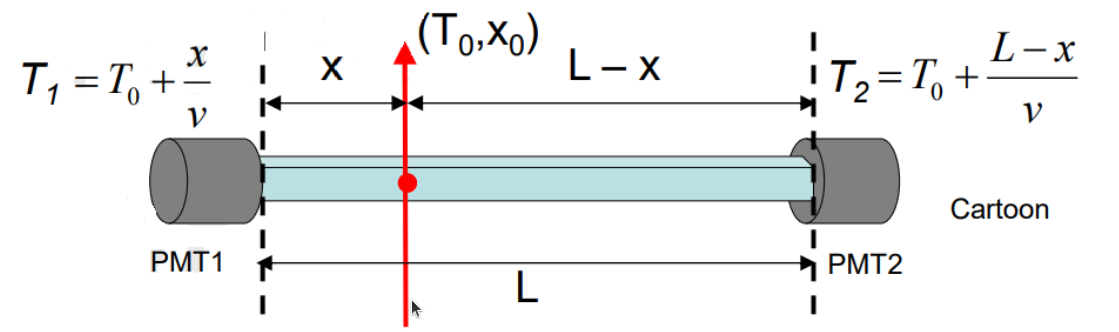
\includegraphics [scale = 0.4] {PHENIX/TOF.png}
	\caption{Схематическое изображение сегмента времяпролетной камеры (TOF)} 
	\label{img:PHENIX_TOF}
\end{figure}

Система TOF состоит из 10 панелей, каждая из которых содержит 96 сегментов, световоды и механические опоры. Схематическое изображение одной из панелей TOF представлено на Рисунке \ref{img:PHENIX_TOF}. Сегмент TOF представляет собой планку сцинтиллятора с фотоумножителями, расположенными на ее концах. Сцинтилляционные планки и световоды обернуты тонкой алюминиевой фольгой и приклеены к доске, имеющей структуру сот. 

\subsection{Глобальные детекторы столкновений}
Время, координаты и множественность частиц столкновения определяются счетчиками пучков (Beam-Beam Counters -- BBC), детектором множественности/вершины (Multiplicity Vertex Detector -- MVD) и калориметрами ZDC (Zero Degree Calorimeters), расположенными вдоль оси пучка. BBC счетчики позволяют измерять как время взаимодействия, так и $z$-координату столкновения. Также ВВС счетчики служат для измерения центральности (см. Раздел \ref{sect3:centr}). MVD предназдначен для измерения множественности частиц, координаты вершины столкновения и флуктуаций в распределении заряженных частиц. ZDC также могут быть использованы для определения центральности, вершины и времени столкновения.

В данной работе из глобальных детекторов был использован только BBC счетчик.

\subsubsection{BBC счетчик}
BBC счетчики предназначены для измерения времени столкновения и его координаты вдоль оси $z$ ($z_{vtx}$), сонаправленной с осью пучка. Поскольку среднеквадратичное значение продольного размера сгустка пучка на RHIC для столкновений Au+Au составляет 25 см, временной разброс ядерных столкновений может достигать 2 нс.

BBC состоит из двух одинаковых счетчиков, окружающих трубу пучков и расположенных на расстоянии 1,44 м от точки взаимодействия вдоль линии столкновения (один с северной стороны, другой с южной стороны). Такое расположение соответствует диапазону псевдобыстрот от 3,0 до 3,9 по полному азимуту. Каждый счетчик BBC состоит из 64 черенковских счетчиков, расположенных радиально вокруг трубы пучков и однодюймовых динодных фотоумножителей (ФЭУ) HAMAMATSU R6178, установленных на 3-сантиметровом кварцевом радиаторе.

Счетчики BBC измеряют время регистрации ведущих заряженных частиц от столкновения. Время столкновения определяется как среднее время регистрации ведущих заряженный частиц в северном и южном счетчике BBC. 
Разница во времени между регистрацией ведущих частиц в северном и южном счетчиках BBC позволяет определить координату вершины столкновения вдоль оси луча. Координата $z_{vtx}$ вершины взаимодействия и количество сработавших ФЭУ в каждом BBC счетчике рассчитываются онлайн и отправляются в триггер первого уровня LVL1. Необходимыми условиями срабатывания LVL1 триггера является детектрирование сигнала в двух или более ФЭУ в каждом ВВС счетчике и попадание $z$-координаты вершины столкновения в диапазон $|z_{vtx}|$ < 20 см.  Эффективность триггера в отношении неупругих столкновений A+B оценивается с помощью Мноте-Карло моделирования детектора PHENIX для создания столкновений A+B в качестве входных данных и составляет 92 ± 2\%. Суммарный заряд, зарегистрированный в BBC используется для определения центральности. Подробное описание измерения центральности приводится в Разделе \ref{sect3:centr}.

